\section*{Consulta 1: Cantidad de atletas registrados por disciplina}

\subsection*{Descripción}
En primera instancia es importante ver que en esta consulta lo que se busca obtener, es el número de atletas que participan en cada disciplina. De esta forma, esta consulta es útil para entender la popularidad de cada disciplina y la distribución de los atletas.

\textbf{SQL}

\begin{verbatim}
SELECT 
    d.NombreDisciplina,
    COUNT(p.IDAtleta) AS NumParticipantes
FROM 
    Disciplina d
JOIN 
    Participa p ON d.IDDisciplina = p.IDDisciplina
GROUP BY 
    d.NombreDisciplina
ORDER BY 
    NumParticipantes DESC;
\end{verbatim}

\begin{center}
    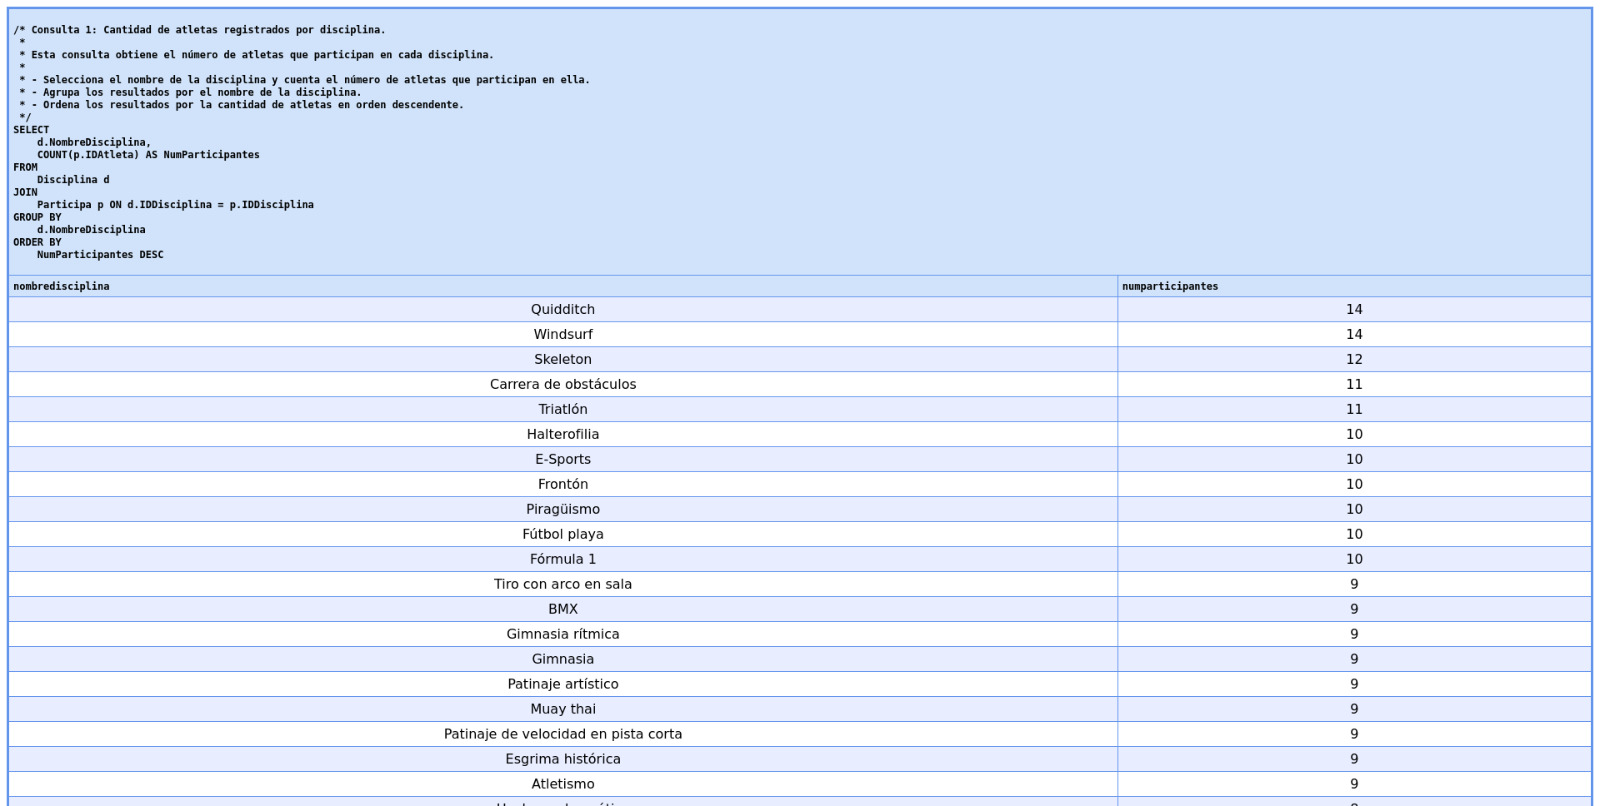
\includegraphics[width=16.5cm]{../resources/Chapters/Consultas/Imagenes/Consulta1.jpeg} 
    
   Consulta 1. Imagen de una parte de la Cantidad de atletas registrados por disciplina.
\end{center}

\textbf{Desglose de la consulta}

\begin{itemize}
   \item \textbf{Selección de columnas (\texttt{SELECT})}:
   \begin{itemize}
       \item Se seleccionan las siguientes columnas de la disciplina:
       \begin{itemize}
           \item \texttt{d.NombreDisciplina}: Nombre de la disciplina.
       \end{itemize}
       \item Se utiliza la función agregada \texttt{COUNT(p.IDAtleta)} para contar cuántos atletas están asociados con cada disciplina. Esta columna se denomina \texttt{NumParticipantes}.
   \end{itemize}
   
   \item \textbf{Tablas involucradas (\texttt{FROM} y \texttt{JOIN})}:
   \begin{itemize}
       \item La consulta utiliza dos tablas:
       \begin{itemize}
           \item \texttt{Disciplina (d)}: Contiene la información de las disciplinas.
           \item \texttt{Participa (p)}: Contiene la información de los atletas que participan en cada disciplina.
       \end{itemize}
       \item Se realiza un \texttt{JOIN} entre ambas tablas utilizando la relación \texttt{d.IDDisciplina = p.IDDisciplina}. Esto asegura que solo se consideren los atletas que están asignados a una disciplina.
   \end{itemize}
   
   \item \textbf{Agrupación de resultados (\texttt{GROUP BY})}:
   \begin{itemize}
       \item Para calcular la cantidad de atletas por disciplina, se agrupan los datos según las columnas únicas de la disciplina:
       \begin{itemize}
           \item \texttt{d.NombreDisciplina}.
       \end{itemize}
       \item Esto garantiza que se genere un registro único por cada disciplina.
   \end{itemize}
   
   \item \textbf{Ordenamiento de resultados (\texttt{ORDER BY})}:
   \begin{itemize}
       \item Los resultados se ordenan por la columna \texttt{NumParticipantes} en orden descendente (\texttt{DESC}), de modo que las disciplinas con más atletas aparezcan primero.
   \end{itemize}
\end{itemize}

\textbf{Análisis detallado}

\begin{enumerate}
   \item \textbf{Relación entre tablas:}
   \begin{itemize}
       \item La consulta asume que existe una relación directa entre las tablas \texttt{Disciplina} y \texttt{Participa} a través de la clave foránea \texttt{p.IDDisciplina}, que apunta a \texttt{d.IDDisciplina}.
       \item Esto implica que:
       \begin{itemize}
           \item Cada atleta está asignado a exactamente una disciplina.
           \item Una disciplina puede tener asignados uno o más atletas.
       \end{itemize}
   \end{itemize}
   
   \item \textbf{Uso de la función agregada \texttt{COUNT}:}
   \begin{itemize}
       \item La función \texttt{COUNT(p.IDAtleta)} cuenta el número de registros en la tabla \texttt{Participa} que están relacionados con cada disciplina.
       \item Si una disciplina no tiene atletas asignados, no aparecerá en los resultados porque el \texttt{JOIN} elimina las filas sin coincidencias.
   \end{itemize}
   
   \item \textbf{Agrupación por disciplina:}
   \begin{itemize}
       \item El uso de \texttt{GROUP BY} permite agrupar los registros por disciplina, asegurando que la cantidad de atletas se calcule correctamente para cada una.
   \end{itemize}
   
   \item \textbf{Ordenamiento:}
   \begin{itemize}
       \item El orden descendente por \texttt{NumParticipantes} facilita la identificación de las disciplinas con mayor número de atletas.
   \end{itemize}
\end{enumerate}

\textbf{Consideraciones}

\begin{itemize}
   \item \textbf{Empates en la cantidad de atletas:}
   \begin{itemize}
       \item Si varias disciplinas tienen la misma cantidad de atletas, el orden relativo entre ellas no está definido. Para resolver esto, se podría agregar un criterio adicional en el \texttt{ORDER BY}, como el nombre de la disciplina.
   \end{itemize}
\end{itemize}